\documentclass[12pt]{article}

\usepackage{cmap} % Улучшенный поиск русских слов в полученном pdf-файле
\usepackage{ucs}
\usepackage[T2A]{fontenc} % Поддержка русских букв
\usepackage[utf8x]{inputenc} % Включаем поддержку UTF8
\usepackage[russian]{babel}  % Включаем пакет для поддержки русского языка

\usepackage{amsfonts}
\usepackage{amsmath}
\usepackage{graphicx}
\usepackage{wrapfig}
\usepackage{float}
\usepackage{caption}
\usepackage{subcaption}

\usepackage{cite}
\usepackage{indentfirst} % Красная строка

\newcommand {\mys}[1]{$\spadesuit$ #1\\}
\newcommand {\mysl}[1]{$\spadesuit$ #1}
\newcommand {\mysf}[1]{\\$\spadesuit$ #1\\}

\usepackage{geometry} % see geometry.pdf on how to lay out the page. There's lots.
\geometry{a4paper} % or letter or a5paper or ... etc
% \geometry{landscape} % rotated page geometry

% See the ``Article customise'' template for come common customisations

\title{Это же дипломная работа,\\к которой вы шли пять лет!}

\author{Герасимов К.\\ \\Руководитель Косенко И.И.}
\date{} % delete this line to display the current date

\begin{document}

\thispagestyle{empty}
\newpage
\begin{centering}

\textbf{
МОСКОВСКИЙ ГОСУДАРСТВЕННЫЙ УНИВЕРСИТЕТ\\
ИМЕНИ М.В. ЛОМОНОСОВА\\*
Механико-математический факультет\\
Кафедра теоретической механики и мехатроники}

\begin{figure}[h]
\centering
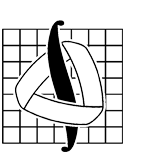
\includegraphics[width=4cm]{mmlogo.png}
\end{figure}
\bigskip
\bigskip

{\Huge ДИПЛОМНАЯ РАБОТА}

\bigskip
\bigskip

{\LARGE Модель динамики омниэкипажа}
\bigskip
\bigskip

{\LARGE Omni-vehicle dynamical model}

\medskip

\bigskip

студента 521 группы\medskip

Герасимова Кирилла Вячеславовича\\
\medskip

\vfill

\begin{flushright}
Научный руководитель: \\
д. ф.-м. н. профессор И. И. Косенко\\



\end{flushright}
\bigskip
\bigskip
\vspace{\fill}
\vspace{\fill}
\vspace{\fill}
\vspace{\fill}

Москва \number\year
\clearpage




\bigskip
\end{centering}

\tableofcontents
\newpage

\section{Введение}

В работе рассматривается подход к физически-ориентированному моделированию экипажа с омниколесами с использованием технологии Modelica.\\

Омниколесо - это колесо, на ободе которого расположены ролики. Имеются оси, закрепленные на колесе, а сами ролики свободно вращаются вокруг этих осей. В отечественной литературе такие системы называют также роликонесущими колесами.\\

Литература, в связи с тем, что рассматриваемый вид колес изобретен не столь давно, не слишком обширна. Теоретические исследования динамики ограничиваются модельными неголономными постановками, не учитывающими, в частности, динамику роликов \cite{kos1,kos2,kos3,kos4}. Говоря точнее, эти подходы предлагают считать ролики бесконечно малыми и "распределять", таким образом, неголономную связь "равномерно" по всему ободу колеса. В результате они приближенно описывают сложную систему - омниколесо - как идеализированный объект с меньшим количеством степеней свободы и иной геометрией масс и динамикой. Представлены \cite{practical, particle} практические работы, авторы которых рассматривают сконструированные ими же экипажи и исследуют вопросы управления их движением. Изучение физических моделей, принимающих во внимание динамику всех частей омни-экипажа (в том числе, роликов), затруднено резким ростом количества степеней свободы системы при увеличении количества роликов на колесе (см. раздел Модель экипажа).\\

Наша цель здесь - построить численную модель динамики омниколесного экипажа на горизонтальной плоскости, учитывающую динамику платформы экипажа, колес и роликов. Мы пренебрегаем трением в шарнирах и принимаем модель кулоновского трения в контакте с плоскостью. Мы используем и расширяем ранее представленную \cite{kos5} библиотеку трехмерной динамики систем тел. Особое значение для данной реализации имеет применяемый способ представления односторонней связи.

\section{Обзор}

Об омниколесах, как таковых, существует немало работ, описывающих и кинематику и динамику. Существуют различные типы омниколес, отличающиеся конфигурацией роликов, количеством точек контакта. К примеру, интересный тип колес - меканум-колеса (см. рис.~\ref{fig:bor_wheel_pic}) - описан в \cite{mecanum}. Данная работа описывает различные варианты геометрической формы поверхности роликов, например, приближения ее сегментами тора, а также исследует прямую (даны скорости вращения колес, получить траекторию центра масс экипажа) и обратную (получить программные скорости вращения колес для заданной траектории) задачи кинематики для экипажа с тремя меканум-колесами в неголономной постановке.\\

\begin{figure}
\centering
\begin{minipage}{.47\textwidth}
    \centering
    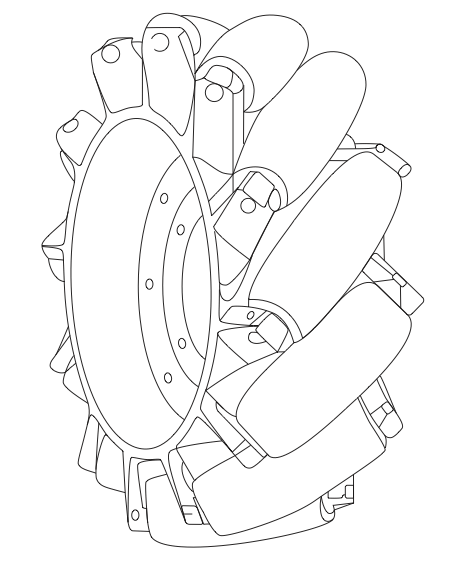
\includegraphics[width=\textwidth]{content/parts/3_friction/diploma/img/art/bor_wheel_pic.png}
    \caption{Меканум-колесо}
    \label{fig:bor_wheel_pic}
\end{minipage}%
\hspace{5pt}
\begin{minipage}{.47\textwidth}
    \centering
    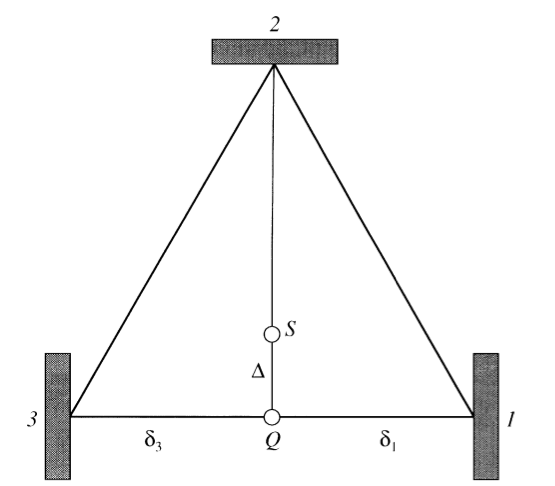
\includegraphics[width=\textwidth]{content/parts/3_friction/diploma/img/art/zobova.png}
    \caption{Конфигурация из \cite{kos4}}
    \label{fig:zobova}
\end{minipage}
\end{figure}

Из работ, рассматривающих движение омниэкипажей в неголономной постановке, следует отметить \cite{kos4,formalskii,borisov}. Во всех трех работах колеса считаются твердыми дисками. В \cite{kos4,borisov} изучаются экипажи произвольной конфигурации, в то время как \cite{formalskii} принимает симметричную трехколесную. \cite{kos4} проводит полный качественный анализ свободного движения экипажа, а также рассматривает, в частности, вопросы управления и устойчивости некоторых движений в конфигурации, приведенной на рис.~\ref{fig:zobova}. Вариант тележки из \cite{formalskii} имеет ролики в плоскостях соответствующих колес. Рассмотрено свободное движение и движение под действием трех постоянных управляющих моментов в осях колес. Исследуется вопрос об энергетической эффективности такого управляемого движения и находится оптимальное положение вектора скорости в теле платформы экипажа для прямолинейного движения. Также затрагивается проблема оценки координат робота при управлении. Работа\cite{borisov} рассматривает свободное движение экипажа на плоскости и сфере, приводит, как и \cite{kos4}, свой вариант вывода общих уравнений движения. Находит некоторые интегралы приведенной (обезразмеренной) системы и исследует ее характерные неподвижные точки, периодические и асимптотические траектории, получая, в частности, явный вид абсолютного движения в этих случаях. Данная работа предлагает также использование омниэкипажа как транспортного средства путем помещения его в сферу и получает уравнения движения на сфере. Построенная модель для плоскости использована нами для верификации нашей объектно-ориентированной компьютерной модели, так как она является новейшим из предложенных неголономных вариантов и учитывает опыт авторов прошлых лет. Подробнее см. раздел Верификация.\\

Говоря о компьютерных моделях, выделим \cite{practical}, использующую технологию объектно-ориентированного моделирования Modelica для построения физической модели омниэкипажа с нелинейной моделью трения в контакте. Она, однако, предполагает, что колесо не может создавать силу трения, ортогональную оси закрепления роликов. Производятся также расчеты управляемого движения для случаев тележки с четырьмя меканум-колесами и симметричной трехколесной конфигурации. Тот же автор исследует в \cite{kos2} поведение экипажа при резком торможении - важный в технике случай - и демонстрирует с использованием своей численной модели появление заноса, возникающего из-за неравномерного распределения силы нормальной реакции при указанном управлении. \cite{kos3} представляет краткое описание одной модели меканум-колеса, применяемой компанией Kuka \cite{kos2}. С помощью Dymola авторы исследуют преодоление четырехколесной платформой вертикального препятствия и поведение нормальной силы реакции в этом случае. \cite{particle} подробно занимается вопросом навигации омниколесного экипажа и описывает использование фильтра частиц для решения задачи определения координат тележки в пространстве. Также автор представляет сконструированный им экипаж и систему управления.

\section{Постановка задачи.\newline Построение физически-ориентированной компьютерной модели}

При построении модели омниэкипажа мы учитываем, что её основные параметры - количество роликов на каждом колесе и угол наклона оси симметрии ролика к плоскости колеса. Для простоты и наглядности рассмотрим омниколесо с четырьмя роликами. Кроме того, для простоты оси симметрии самих роликов расположим в плоскости колеса см. рис.~\ref{fig:kos1_wheel_side}. Эти основные параметры достаточно легко изменять. Будем считать также, что ролики расположены на колесе таким образом, что проекция кривой контакта - внешней границы колеса вместе с роликами - на плоскость колеса представляет собой последовательность неперекрывающихся сегментов, каждый из которых соответствует некоторому ролику. Эти сегменты связаны таким образом, например, что нормальная относительная скорость в контакте равна нулю в момент переключения роликов. Благодаря этому, нормальные удары отсутствуют. Касательная составляющая скорости относительного скольжения непрерывна при нулевом угле наклона осей роликов к плоскости колеса. Однако касательная сила трения может иметь разрыв в худшем случае первого рода, если ось симметрии ролика наклонена к плоскости колеса. Таким образом, линейная и угловая скорости колеса непрерывны в момент переключения контакта ролика. Аналогичное утверждение верно также и для роликов. Тогда касательные удары также отсутствуют.\\

\begin{figure}
\centering
\begin{minipage}{.47\textwidth}
    \centering
    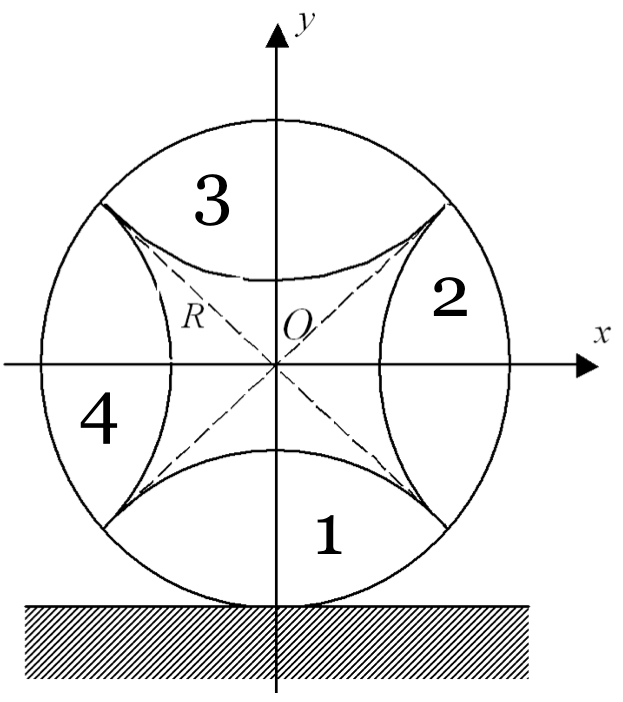
\includegraphics[width=\textwidth]{content/parts/3_friction/diploma/img/art/kos1_wheel_side.png}
    \caption{Вертикально расположенное омниколесо}
    \label{fig:kos1_wheel_side}
\end{minipage}%
\hspace{5pt}
\begin{minipage}{.47\textwidth}
    \centering
    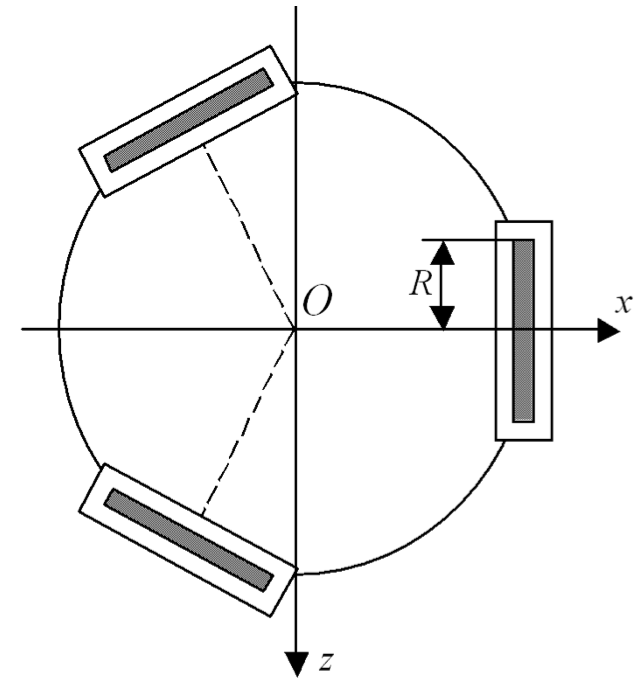
\includegraphics[width=\textwidth]{content/parts/3_friction/diploma/img/art/kos2_vehicle.png}
    \caption{Трехколесный экипаж, вид сверху}
    \label{fig:kos2_vehicle}
\end{minipage}
\end{figure}


Отметим дополнительно, что кривая, образуемая возможными точками контакта, в проекции на плоскость колеса является окружностью радиуса $R$, см. рис.~\ref{fig:kos1_wheel_side}. Таким образом, поступательное и вращательное движение непрерывны. Окончательно можем заключить, что движение остается невырожденным в момент переключения контакта с одного ролика на другой, по крайней мере, когда колесо вертикально.\\

Переходя на следующий структурный уровень, рассмотрим несколько омниколес, соединенных с движущейся платформой экипажа (см. рис.~\ref{fig:kos2_vehicle}), посредством шарнирной связи. Эта последняя реализуется как класс в смысле языка Modelica, представленный ранее \cite{kos5}. В нашем случае количество колес может быть три или больше. Они могут располагаться на платформе в разных конфигурациях. Мы рассматриваем здесь, для примера, систему с тремя колесами, расположенными в вершинах правильного треугольника, лежащего в плоскости платформы (см. рис.~\ref{fig:kos2_vehicle}), параллельной координатной плоскости $ZX$. Ось $Y$ полагаем вертикальной.\\

\subsection{Динамическая модель ролика}

Мы называем роликом осесимметричное твердое тело в форме веретена, поверхность которого задается в осях $Oxyz$, связанных с телом (см. рис.~\ref{fig:kos3_roller_frame}) уравнением
\begin{equation}
    x^2 + (\sqrt{y^2+z^2} + R_1)^2 = R,
\end{equation}
где $R$ - внешний радиус омниколеса, $R_1 = R\cos\alpha$ - расстояние от центра ролика до центра колеса, $\alpha = \frac{\pi}{n}$ - половина угла с вершиной в центре колеса, опирающегося на дугу ролика, $n$ - количество роликов на колесе.\\

\begin{figure}[h]
    \centering
    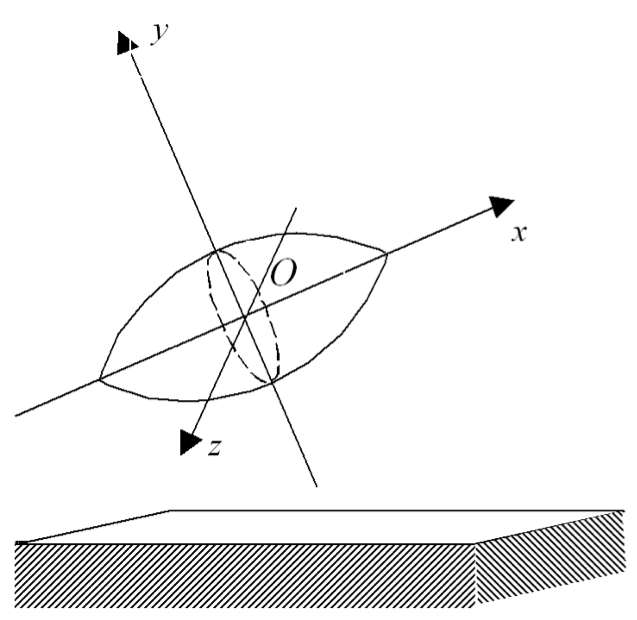
\includegraphics[width=0.4\textwidth]{content/parts/3_friction/diploma/img/art/kos3_roller_frame.png}
    \caption{Ролик на горизонтальной плоскости}
    \label{fig:kos3_roller_frame}
\end{figure}

Динамика поступательно-вращательного движения реализуется в численной модели с помощью уравнений Ньютона-Эйлера \cite{kos6}. Ориентация ролика в пространстве представляется кватернионами \cite{kos7}.\\

\subsection{Отслеживание контакта}

Алгоритм отслеживания точки контакта играет важнейшую роль для точности и вычислительной эффективности компьютерной модели процесса контактирования ролика и горизонтальной плоскости. Для моделирования и симуляции динамики твердого тела с односторонней связью мы применяем технологию из \cite{kos8}. Возможно применять систему известных неявных дифферен\-циально\--алгебраических уравнений при реализации объекта, отслеживающего контакт на Modelica. Однако эти уравнения вырождаются в вершинах роликов $x = \pm R\sin\alpha$ (в локальных для ролика координатах, см. рис.~\ref{fig:kos1_wheel_side}). Как правило, подобное вырождение приводит к аварийному завершению процесса симуляции.\\

\begin{figure}[h]
    \centering
    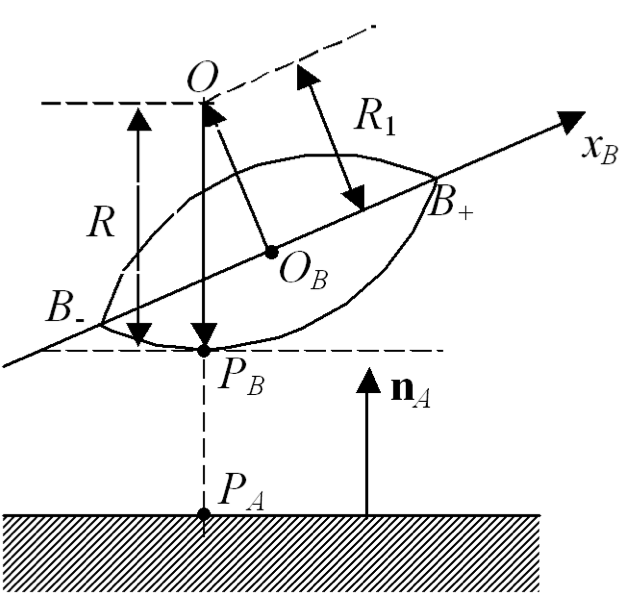
\includegraphics[width=0.5\textwidth]{content/parts/3_friction/diploma/img/art/kos4_roller_contact.png}
    \caption{Схема отслеживания контакта}
    \label{fig:kos4_roller_contact}
\end{figure}

В рассматриваемом случае ролика-веретена на горизонтальной плоскости оказывается возможно устроить процедуру отслеживания точки контакта достаточно простым способом. Можно указать явный способ вычисления ближайшей к горизонтальной плоскости точки ролика $P_B$ (см. рис.~\ref{fig:kos4_roller_contact}). Ближайшая же к ролику точка плоскости $P_A$ является, очевидно, вертикальной проекцией точки ролика $P_B$ на плоскость.\\

Обозначим $\vec{i} = (1,0,0)^T$ единичный вектор вдоль оси $O_Bx_B$ системы координат, связанной с роликом (рис.~\ref{fig:kos4_roller_contact}), записанный в осях $O_Bx_By_Bz_B$. Пусть $T_B$ - матрица поворота от инерциальной системы координат к осям ролика. Первая в нашем случае совпадает с неподвижными осями $O_Ax_Ay_Az_A$, связанными с плоскосью. Также, пусть $\vec{r_B}$ - координаты центра масс ролика в неподвижных осях, и $\vec{n_A} = (0,1,0)^T$ - вектор восходящей нормали к горизонтальной плоскости.\\

Примем обозначения для тел: $A$ - для плоскости, $B$ - для ролика. Пусть $\vec{d}$ - горизонтальный единичный вектор, определяемый как
$$\vec{d} = \frac{T_B\vec{i_B}\times\vec{n_A}}{\vert T_B\vec{i_B}\times\vec{n_A}\vert}.$$

Таким образом, вектор $\vec{O_BO}$ должен иметь длину $R_1$, и определяться как
$$\vec{O_BO} = R_1\vec{d}\times T_B\vec{i_B}.$$

Здесь O - центр кривизны дуги, образующей одну сторону вертикального сечения ролика (см. рис.~\ref{fig:kos4_roller_contact}). Этот вектор лежит в плоскости колеса и в вертикальной плоскости. Таким образом, из рис.~\ref{fig:kos4_roller_contact} очевидно, что точка $P_B$ поверхности ролика - это
\begin{equation}
\label{rPB}
\vec{r_{P_B}} = \vec{r_B} + R_1\vec{d}\times T_B\vec{i_B}-R\vec{n_a},
\end{equation}
поскольку $P_B$ лежит на одной вертикальной прямой с точкой $O$. Координаты $P_A$ тогда
\begin{equation}
\vec{r_{P_A}} = (x_{P_B},0,z_{P_B})^T.
\end{equation}

Описанная процедура верна лишь если угол наклона $T_B\vec{i_B}$ к горизонтальной плоскости по величине не превосходит $\alpha$. В противном случае надо полагать $P_B = B_-$, где $B_-$ - левая (см. рис.~\ref{fig:kos4_roller_contact}) вершина ролика, в случае, если угол наклона больше $\alpha$, либо $P_B = B_+$, где $B_+$ - правая вершина для угла наклона, меньшего $-\alpha$.\\

И наконец, условие, при котором имеет место контакт между роликом и плоскостью, может быть записано как
\begin{equation}\label{contact_1}
\vert T_B\vec{i_B}\cdot\vec{n_A}\vert\leq\sin\alpha.
\end{equation}

Это условие, однако, выполняется и для самого нижнего, и для самого верхнего ролика одновременно. Чтобы отбросить верхний случай, нужно добавить ещё одно условие:
\begin{equation}\label{contact_2}
y_B<R,
\end{equation}
где $y_B$ - высота центра масс ролика над горизонтальной плоскостью.\\

Таким образом, совокупность условий $\eqref{contact_1}$ и $\eqref{contact_2}$ эквивалентна случаю контакта. В ином случае нужно рассматривать условие равенства силы реакции нулю. Действительно, по принципу Синьорини, для каждого ролика верно одно из двух утверждений: а) ролик в контакте, относительная скорость по нормали равна нулю; и б) контакта нет, реакция (и нормальная, и касательная) равна нулю.\\

Условие а) можно записать различными способами. Например, с геометрической точки зрения, наличие контакта равносильно равенству
\begin{equation}
\label{contact_geom}
y_{P_B} = 0.
\end{equation}
Отсутствие же его эквивалентно
$$F_n = 0,$$
где $F_n$ - нормальная составляющая силы реакции, действующей на ролик в точке $P_B$.\\

Практика вычислений показывает, что уравнение контакта в форме \eqref{contact_geom} вызывает, как правило, аварийное завершение расчета динамической модели ролика. Подобный исход получаем и при использовании формы 
$$v_n = 0,$$
условия а). Здесь $v_n$ - нормальная составляющая относительной скорости в точке контакта. И только уравнение вида 
$$\dot{\vec{v_n}} = 0$$ приводит к искомому результату: объект, реализующий контактное взаимодействие работает правильно в течение всего процесса симуляции. Напомним, что реализация всего процесса контактирования полагает контакт точечным.\\

Для каждого ролика омниэкипажа модель силы трения "включается" на период, когда он находится в контакте. В разработанной модели использован закон трения Кулона-Амонтона. Мы используем известное кусочно-заданное приближение \cite{kos8} точного закона сухого трения. В целом, реализация односторонней связи основана на результатах, представленных в \cite{kos8}.\\

Если угол наклона оси симметрии ролика к плоскости колеса ненулевой, то некоторые соотношения, указанные выше необходимо уточнить. В таком случае форма роликов должна быть растянута вдоль обода колеса. Обозначим положение центра $O$ колеса как $\vec{r_O} \in \Re^3$ (см. рис.~\ref{fig:kos4_roller_contact}). Введем вспомогательный базис 
\begin{equation*}
\vec{i}^{\hspace{2pt}\prime} = T_B \left( \begin{array}{ccc} 1\\0\\0 \end{array}\right),\hspace{10pt}
\vec{j}^{\hspace{1pt}\prime} = \frac{\vec{r_O}-\vec{r_{O_B}}}{\vert\vec{r_O}-\vec{r_{O_B}}\vert},\hspace{10pt}
\vec{k}^\prime = \vec{i}^{\hspace{2pt}\prime}\times\vec{j}^{\hspace{2pt}\prime}.
\end{equation*}

Соответствующая матрица перехода имеет вид $T^\prime = (\vec{i}^\prime\vec{j}^\prime\vec{k}^\prime)$, где $\vec{i}^\prime, \vec{j}^\prime, \vec{k}^\prime$ полагаются векторами-столбцами. Эта матрица определяет
 замену координат от системы отсчета, связанной с телом А, к системе, определяемой базисом $B^\prime = \left\{\vec{i}^\prime,\vec{j}^\prime,\vec{k}^\prime\right\}$ как
$$\left(\begin{array}{ccc}x_A\\y_A\\z_A\end{array}\right) = T^\prime\left(\begin{array}{ccc}x^\prime\\y^\prime\\z^\prime\end{array}\right).$$
 
Чтобы свести анализ к уже рассмотренному выше случаю $\beta = 0$, необходимо повернуть базис $B^\prime$ вокруг оси $\vec{j}^\prime$ на угол $-\beta$ так, что после поворота новый базис $B = \{\vec{i},\vec{j},\vec{k}\}$ будет ориентирован по плоскости колеса, т.е. его векторы $\vec{i}, \vec{j}$ будут лежать в этой плоскости. Этому повороту соответствует матрица 
$$\left(\begin{array}{ccc}
\cos\beta & 0 & -\sin\beta \\
0         & 1 & 0          \\
\sin\beta & 0 & \cos\beta  \\
\end{array}\right)$$
в базисе $B^\prime$. Затем в базисе тела $A$ поворот единичного вектора $\vec{i}^\prime$ представляется как $\vec{i} = T^\prime S(1,0,0)^T$. Положим также $\vec{j} = \vec{j}^\prime, \vec{k} = \vec{i}\times\vec{j}$. Очевидно, $\vec{k} = \vec{d}$, где $\vec{d}$ - единичный вектор, определенный выше.\\

Таким образом, основываясь на выражении \eqref{rPB} и принимая во внимание рис.~\ref{fig:kos4_roller_contact}, можно заключить, что для случая $\beta\neq 0$ имеет место следующий результат:
\begin{equation}
\vec{r_{P_B}} = \vec{r_B}+R_1\vec{j} - R\vec{n_A} - \frac{R_1\tan\beta\sin\gamma}{\sqrt{1-\sin^2\gamma}}\vec{j}\times\vec{i},
\end{equation}
где угол $\gamma$ удовлетворяет уравнению
$$\sin\gamma = \vec{i}\cdot\vec{n_A}.$$

\subsection{Модель экипажа}
Процесс сборки модели экипажа производится в два этапа: а) сборка модели одного омниколеса, содержащего ступицу и ролики; б) сборка всего экипажа посредством создания экземпляров класса омниколеса из п. а) в модели-контейнере, соответствующей экипажу (вместе с остальными необходимыми компонентами).\\

Для соединения роликов, а точнее, объектов класса ролик, со ступицей колеса мы используем модель шарнирной связи, разработанную ранее и представленную в \cite{kos5}. Это класс, представляющий вращение вокруг некоторой наперед заданной оси. Исходный код всех классов и моделей для данной задачи реализован в виде библиотеки языка Modelica. Визуальное представление модели колеса см. на рис.~\ref{fig:kos5_wheel_model}. В этом примере мы приняли, для простоты и ясности $n = 4$.\\

Модель, представляющая основной интерес - это модель всего экипажа, создаваемая на второй стадии описанного процесса. Соединения между колесами и платформой также реализованы в виде класса шарнира из п. а). Эти шарниры допускают вращение без сопротивления вокруг заданной оси и не допускают сдвиг. Визуальное представление модели экипажа - на рис.~\ref{fig:kos6_vehicle_model}. Здесь для ясности изображения объекты даны в виде отдельных экземпляров. На деле же, создаются массивы роликов, колес и шарниров для произвольного $n$ и произвольного количества колес. Таким образом, экипаж имеет $nN+3$ степеней свободы, где $N$ - количество колес, а $3$ соответствует степеням свободы платформы.\\

\begin{figure}[h!]
    \centering
    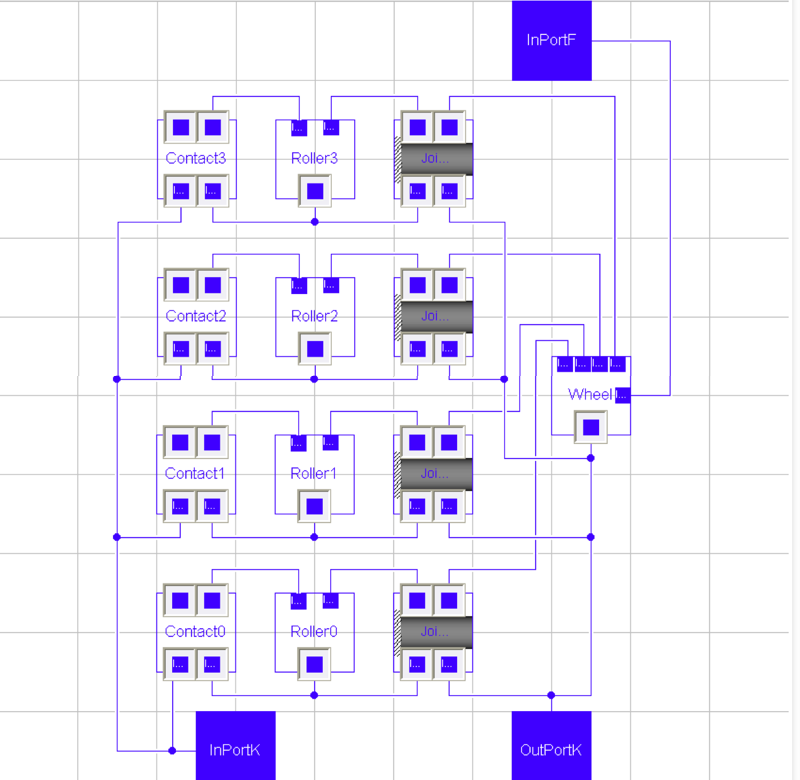
\includegraphics[width=0.85\textwidth]{content/parts/3_friction/diploma/img/art/kos5_wheel_model.png}
    \caption{Визуальная модель омниколеса}
    \label{fig:kos5_wheel_model}
\end{figure}

Моделирование производилось в среде Dymola \cite{DymolaMan}. Перед вычислениями Dymola производит редукцию индекса системы дифферен\-циально\--алгебраичес\-ких уравнений. Модель экипажа до редукции состоит из: а) одного твердого тела - платформы; б) $N$ (трех в рассматриваемом случае) твердых тел - ступиц колес; в) $N\cdot n$ (двенадцати) твердых тел роликов, расположенных на колесах. В соответствии, например, с \cite{kos5}, для каждого объекта твердого тела мы задаем шесть обыкновенных дифференциальных уравнений Нютона движения центра масс и семь ОДУ Эйлера для вращательного движения тела вокруг центра масс. Последние суть четыре кинематических уравнения Эйлера для кватерниона ориентации твердого тела и три уравнения динамики с угловой скоростью. То есть модель экипажа включает систему ОДУ $n(N + 1) \cdot (6+7)$ (16$\cdot$13 = 208) порядка. Кроме этого, объекты связей могут порождать дополнительные дифференциальные уравнения.\\

\begin{figure}[h!]
    \centering
    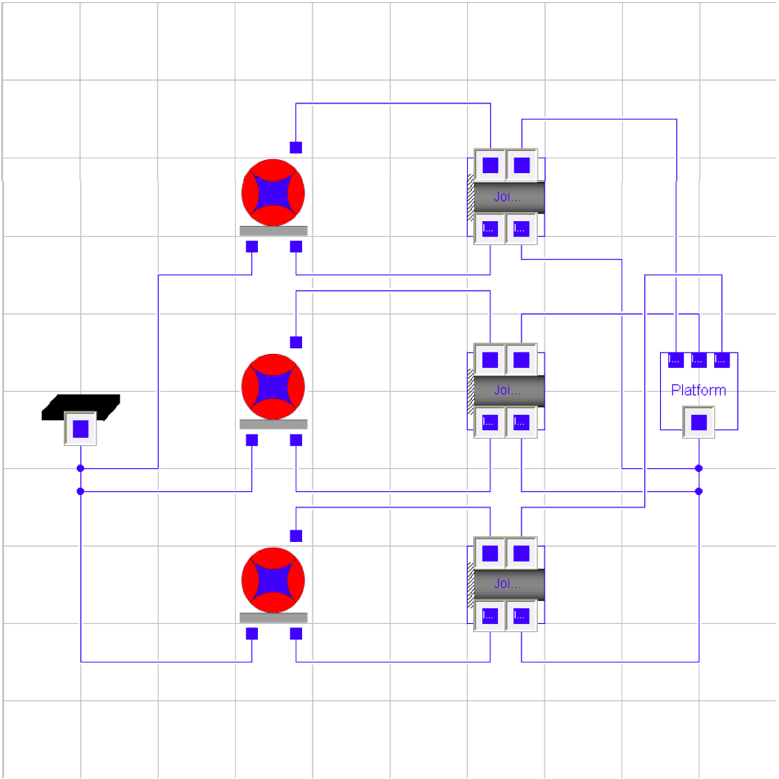
\includegraphics[width=0.95\textwidth]{content/parts/3_friction/diploma/img/art/kos6_vehicle_model.png}
    \caption{Визуальная модель экипажа}
    \label{fig:kos6_vehicle_model}
\end{figure}

Колеса, являющиеся частью экипажа, неизбежно сохраняют вертикальное положение. Благодаря этому свойству алгоритм отслеживания контакта, описанный выше, работает правильно.\\

\section{Верификация}
\subsection{Гипотеза о близости решений}
В литературе представлены \cite{borisov, formalskii, kos4} работы, рассматривающие омниколеса в предположении, что массой и инерцией роликов можно пренебречь, налагающие на систему неголономные связи, ограничивающие направление скорости скольжения в точках контакта колес с поверхностью, на которой стоит экипаж, и не вводящие силу трения в контакте, т.е. считающие скольжение идеальным. Эти идеализированные модели имеют существенно меньше степеней свободы, чем "реальный" омниэкипаж, и легче поддаются аналитическому исследованию.\\

Описанные модели можно использовать для верификации построенной физически-ориентированной модели, рассматривая некоторые элементарные виды движений. Максимальное соответствие построенной модели упомянутым неголономным может быть достигнуто при уменьшении вляиния массы роликов на динамику колеса, а именно, при уменьшении их массы с сохранением общей массы колеса с роликами. На этом предположении и основан наш подход к верификации.\\

\subsection{Проверочная модель}

Для верификации использованы результаты работы \cite{borisov} как новейшей из неголономных моделей динамики свободной тележки с омниколесами на плоскости.\\

Авторы \cite{borisov} принимают простейшую модель омниколеса как плоского диска, для которого скорость точки контакта с опорной поверхностью направлена вдоль прямой, составляющей некоторый угол $\delta$ с плоскостью колеса (см. рис.~\ref{fig:bor_wheel_scheme}). Связь, наложенная на колесо в таком случае имеет вид
$$\vec{v_Q}\cdot\vec{\alpha} = 0,$$
где $\vec{v_Q}$ - скорость точки контакта, $\vec{\alpha}$ - единичный вектор вдоль оси закрепления роликов.\\

\begin{figure}[h!]
    \centering
    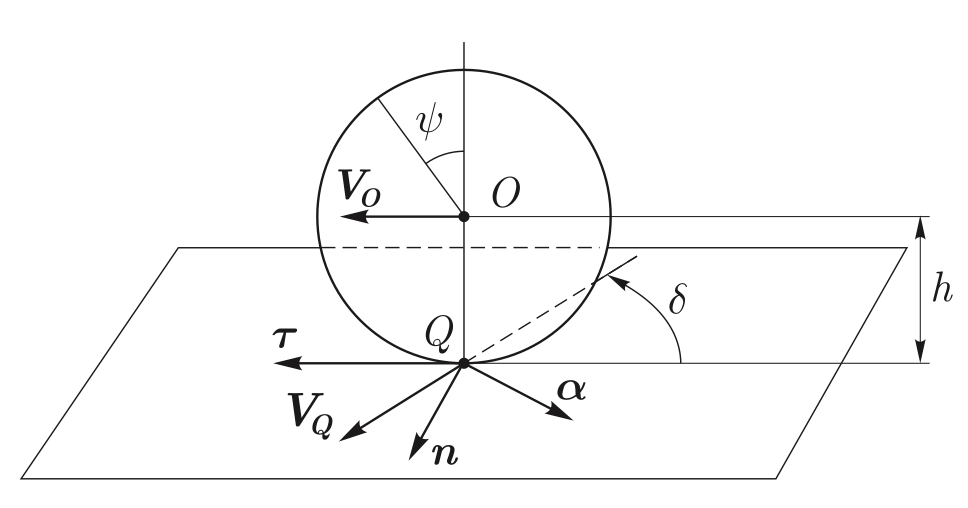
\includegraphics[width=0.75\textwidth]{content/parts/3_friction/diploma/img/art/bor_wheel_scheme.png}
    \caption{Неголономная модель колеса}
    \label{fig:bor_wheel_scheme}
\end{figure}

Авторы \cite{borisov} получают уравнения движения для экипажа с произвольным количеством колес, закрепленных так, что их оси неподвижны относительно платформы, а оси роликов повернуты на произвольные углы относительно плоскостей соответствующих колес (см.рис.~\ref{fig:bor_vehicle}).

\begin{figure}[h!]
    \centering
    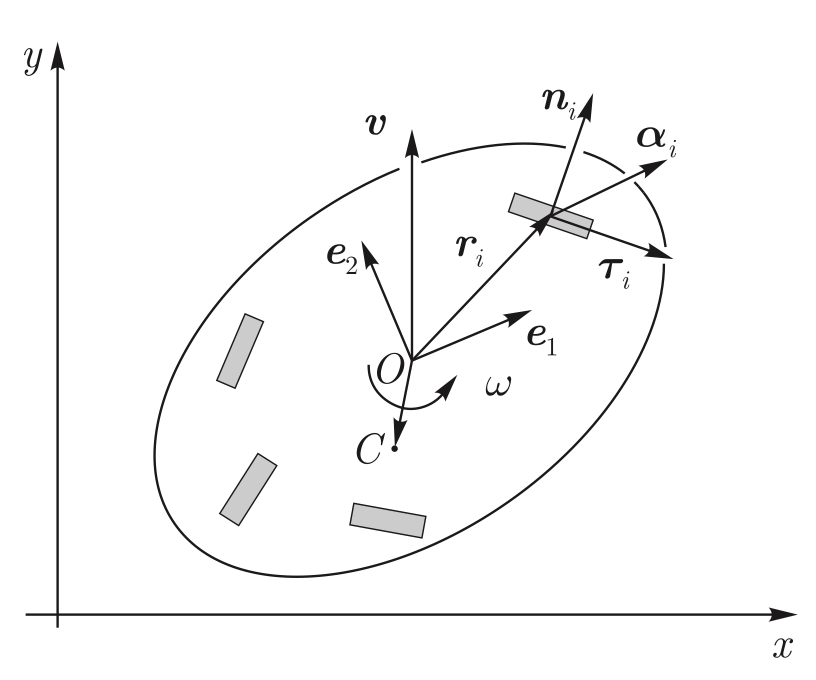
\includegraphics[width=0.75\textwidth]{content/parts/3_friction/diploma/img/art/bor_vehicle.png}
    \caption{Неголономная модель экипажа}
    \label{fig:bor_vehicle}
\end{figure}

Вводится подвижная система отсчета, связанная с платформой экипажа (см.рис.~\ref{fig:bor_vehicle}). Уравнения свободного движения имеют вид:
\begin{eqnarray*}
(\Gamma+mE)\dot{\vec{v}} + m\dot{\omega}(J\vec{r_C}+R)+m\omega J(\vec{v} + \omega J\vec{r_C}) = 0,\\
\hat{I}\dot{\omega} + m(J\vec{r_C}+\vec{r})\cdot\dot{\vec{v}}+m\omega\vec{v}\cdot\vec{r_C} = 0,\\
\dot{x} = v_1\cos\phi - v_2\sin\phi, \dot{x} = v_1\sin\phi + v_2\cos\phi, \dot{\phi} = \omega,\\
\Gamma_{kl} = \sum_i \frac{I_i}{s_i^2 h_i^2}\alpha_i^k\alpha_i^l, R = m^{-1}\sum_i \frac{I_i}{s_i^2 h_i^2}(J\vec{r_i}\cdot \alpha_i) \alpha_i,\\
\hat{I} = I + \sum_i \frac{I_i}{s_i^2 h_i}(J\vec{r_i}\cdot \alpha_i)^2,
\end{eqnarray*}%
\newline
где $\hat{I}$ - суммарный момент инерции системы относительно вертикальной оси, проходящей через начало $O$ подвижной системы отсчета,\newline
$I$ - момент инерции платформы относительно той же прямой,\newline
$I_i$ - моменты инерции колес относительно их диаметров,\newline
$s_i = \sin\delta_i$, $h_i$ - радиусы колес,\newline
$\vec{r_i}$ - точки закрепления осей колес в подвижной системе,\newline
$J = \left(\begin{array}{cc}0 & 1\\-1 & 0\end{array}\right)$,\newline
$x,y,\phi$ - координаты точки $O$ и угол поворота платвормы экипажа вокруг вертикальной оси,\newline
$\vec{v}, \omega$ - вектор скорости точки $O$ и скорость поворота платформы,\newline
$\vec{r_C}$ - координаты центра масс экипажа в подвижных осях,
$E$ - единичная матрица.\\

Данная неголономная модель экипажа также реализована на языке Modelica \cite{ModelicaSpec} как часть упомянутой библиотеки \cite{kos5}. Таким образом, возможно проведение сравнительного анализа физически-ориентированной и идеализированной моделей и верифкация.

\subsection{Два типа движений}
Задавая параметры экипажа, такие как массы его частей, их моменты инерции, геометрические размеры, положения, а также начальные данные - скорость центра масс и угловую скорость платформы, - и выполняя согласованные расчеты для двух реализаций - физической и идеальной - можно получить достаточно близкие движения при достаточно малой доле массы роликов.\\

\begin{figure}[h!]
    \centering
    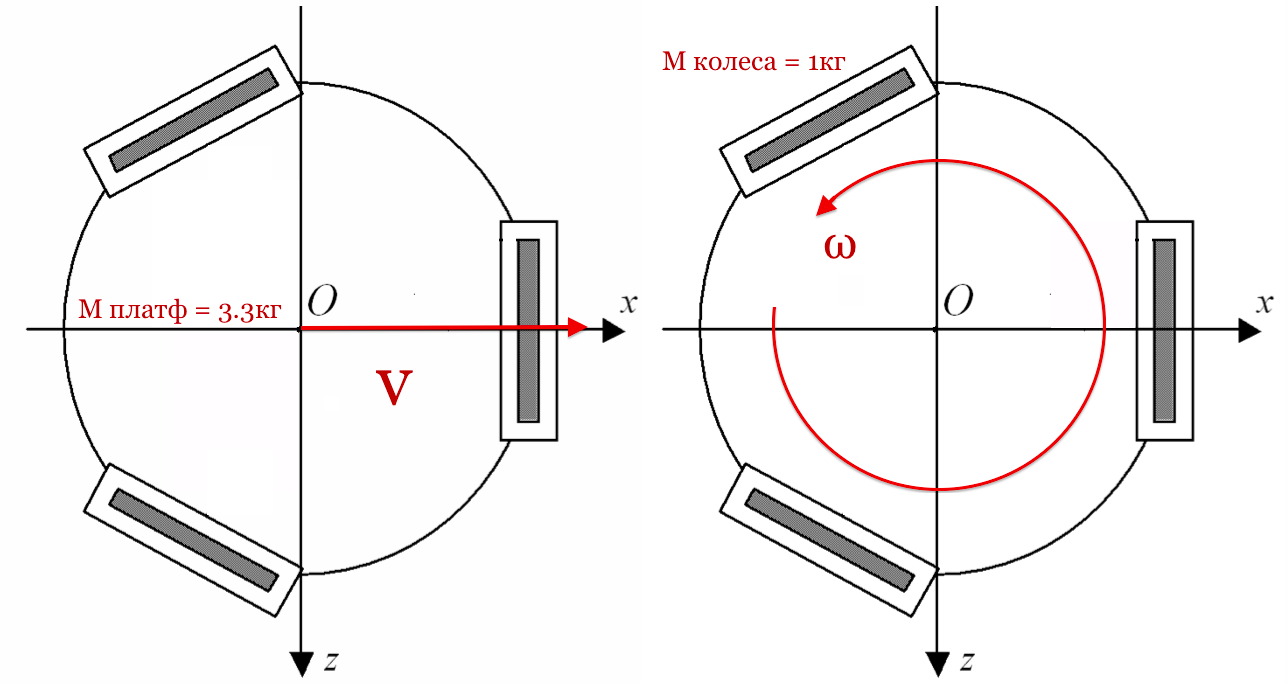
\includegraphics[width=0.95\textwidth]{content/parts/3_friction/diploma/img/art/my_exp_setup.png}
    \caption{Параметры экспериментов}
    \label{fig:my_exp_setup}
\end{figure}

При выполнении численных экспериментов массы платформы и колес, количество колес, количество роликов, геометрия системы были фиксированы (см. рис.~\ref{fig:my_exp_setup}). Изменялись начальные данные и доля массы роликов.\\

Рассмотрены два типа начальных условий $\vec{v}(0) = (v_0, 0, 0)^T, \omega(0) = \omega_0$ (см. рис.~\ref{fig:my_exp_setup}):
\begin{enumerate}
\item экипаж закручен вокруг вертикальной оси, проходящей через его центр масс, скорость центра масс равна нулю (ожидаемый результат - экипаж вращается вокруг своей вертикальной оси симметрии, и центр масс покоится),
\item экипаж имеет начальную линейную скорость в направлении одного из колес и не закручен (ожидаемый результат - центр масс экипажа движется вдоль оси $Ox$, экипаж не вращается).
\end{enumerate}

Значения отношения $\eta$ массы ролика к общей массе колеса принимали в обоих случаях значения от $10^{-6}n^{-1}$ до $10^{-1}n^{-1}$ с шагом $1$ по порядку малости (здесь $n$ - фиксированное количество роликов).

На рис.~\ref{fig:exp_examples} приведены примеры траектории центра масс $y(x)$ и зависимости $\psi(t)$ угла поворота $\psi$ платформы вокруг вертикальной оси, проходящей через её центр, для случаев 1) и 2). Кривые $y(x)$, изображающие траектории центра масс, соответствуют, в сущности, точке - началу координат - в случае $v_0 = 0, \omega_0 = 1$, и отрезку прямой, совпадающей с осью $x$, в случае $v_0 = 1, \omega_0 = 0$, ибо масштаб отображения таков, чтобы были видны отклонения от точных значений, возникающие в силу вычислительной погрешности, но сами эти отклонения имеют порядок малости, позволяющий считать их нулевыми. Аналогичное утверждение верно и для зависимости угла поворота платформы $\psi$ от времени в случае поступательного движения - полученная зависимость близка к постоянной.\\

Ниже представлены результаты нескольких численных экспериментов. Во всех случаях величины, изображенные на рис.~\ref{fig:exp_examples}, демонстрируют поведение, не различимое в масштабе рис.~\ref{fig:exp_examples}, и поэтому приведены лишь расхождения между построенной нами моделью и верификационной идеализацией, которые и представляют интерес. Также представлена абсолютная величина скорости скольжения в точке контакта в физической модели.\\

Графики зависимости скорости скольжения от времени показывают, что скольжение имеет место в окрестности момента смены роликов. Это объясняется тем, что для идеального качения в эти моменты ролику необходима бесконечная угловая скорость собственного вращения, ибо его размер вблизи вершины стремится к нулю. Видно, что с ростом доли массы роликов в общей массе колеса скольжение в контакте становится существеннее, изменяясь от пренебрежимо малого при $\eta = 10^{-6}$ до весьма существенного уже при $\eta = 10^{-3}$. Тем не менее, расхождения траектории и угла поворота платформы малы, а скольжение наблюдается лишь в точках колеса, которые в промышленных конструкциях не присутствуют (см. Обзор), что и позволяет считать верификацию проведенной.

% EXAMPLES
\begin{figure}[h!]
\centering
\begin{subfigure}{.47\textwidth}
    \centering
    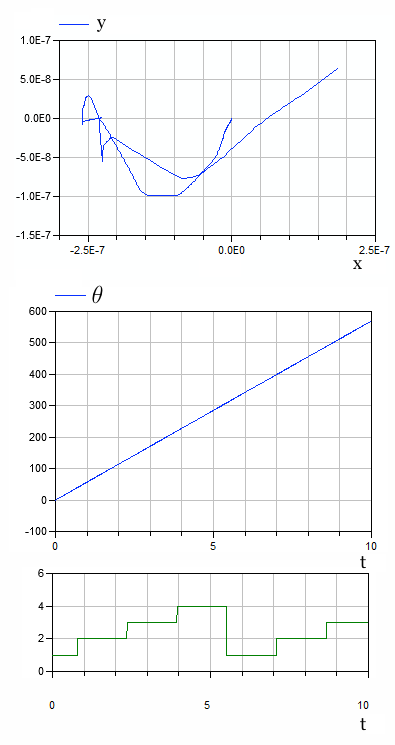
\includegraphics[width=\textwidth]{content/parts/3_friction/diploma/img/res/example_v_0_0_omega_1_frac_1e-1_n_4_time_10s.png}
    \caption{$\eta = 0,1, v_0 = 0, \omega_0 = 1$}
    \label{fig:exp_example_omega}
\end{subfigure}%
\hspace{5pt}
\begin{subfigure}{.47\textwidth}
    \centering
    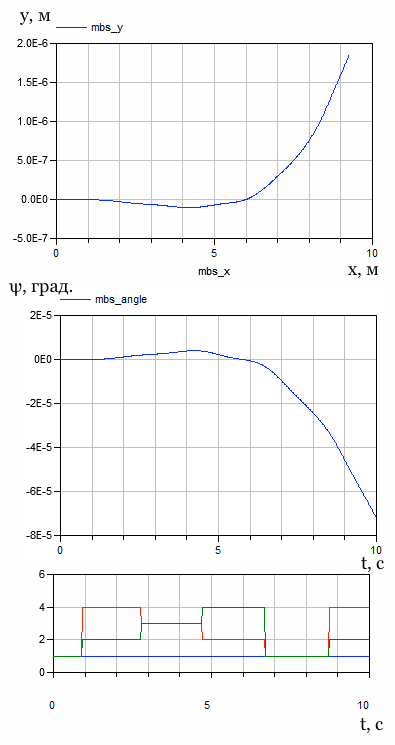
\includegraphics[width=\textwidth]{content/parts/3_friction/diploma/img/res/example_v_1_0_omega_0_frac_1e-1_n_4_time_10s.png}
    \caption{$\eta = 0,1, v_0 = 1, \omega_0 = 0$}
    \label{fig:exp_example_v}
\end{subfigure}
\caption{Примеры траекторий, характера изменения угла и смены номеров роликов в контакте для двух типов начальных условий. На нижнем графике - номер ролика в контакте, см. рис.~\ref{fig:kos1_wheel_side}}
\label{fig:exp_examples}
\end{figure}



\section{Выводы и дальнейшая работа}

Построена объектная физически-ориентированная модель экипажа с омниколесами, проведена верификация - сравнение с неголономной моделью экипажа, также реализованной в рамках подхода объектно-ориентированного моделирования.\\

Верификация показывает близость решений в указанных моделях на основных примерах начальных данных и практически полное совпадение при соответствующем уменьшении доли массы роликов в общей массе колеса, при использовании модели трения Кулона-Амонтона и симметричной трехколесной конфигурации экипажа.\\

Представляет интерес реализация иных, более точных моделей контакта (например, модели Герца) и проведение численных экспериментов для иных конфигураций экипажа (например, с четырьмя меканум-колесами). Конечным применением моделей, основанных на данной, может стать использование их для управления реальными экипажами.

\bibliographystyle{utf8gost705u}  %% стилевой файл для оформления по ГОСТу
\bibliography{biblio}     %% имя библиографической базы (bib-файла) 




\begin{figure*}[p]
\begin{center}\begin{equation*}\begin{array}{cc}
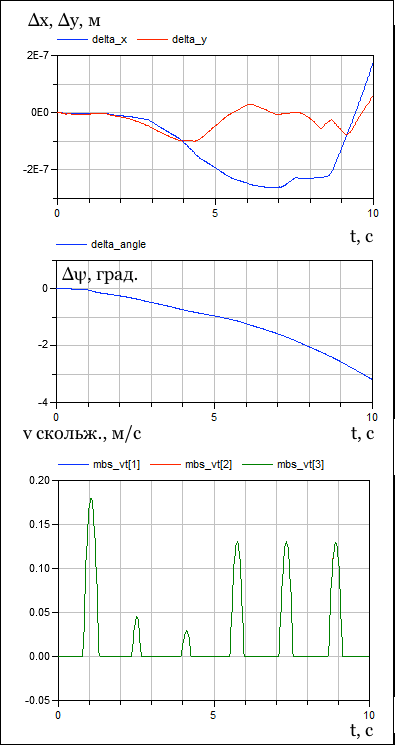
\includegraphics[width=7cm, viewport=0 0 395 745,clip]{content/parts/3_friction/diploma/img/res/comparison_v_0_0_omega_1_frac_1e-1_n_4_time_10s.png} & 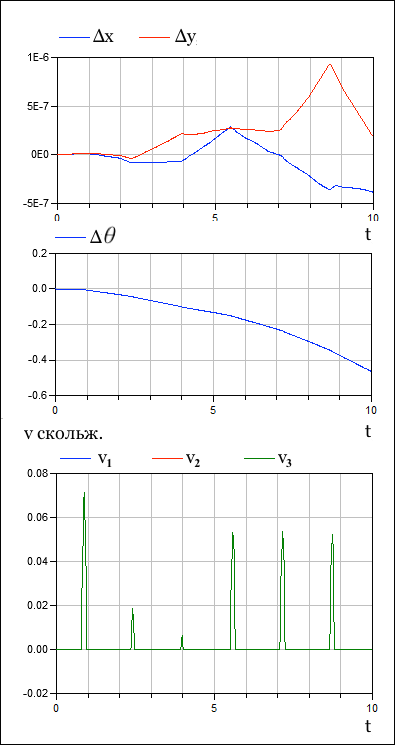
\includegraphics[width=7cm, viewport=0 0 395 745,clip]{content/parts/3_friction/diploma/img/res/comparison_v_0_0_omega_1_frac_1e-2_n_4_time_10s.png}\\
\eta = 0,1, v_0 = 0, \omega_0 = 1 & \eta = 0,01, v_0 = 0, \omega_0 = 1\\
\end{array}\end{equation*}\end{center}
\end{figure*}

\begin{figure*}[p]
\begin{center}\begin{equation*}\begin{array}{cc}
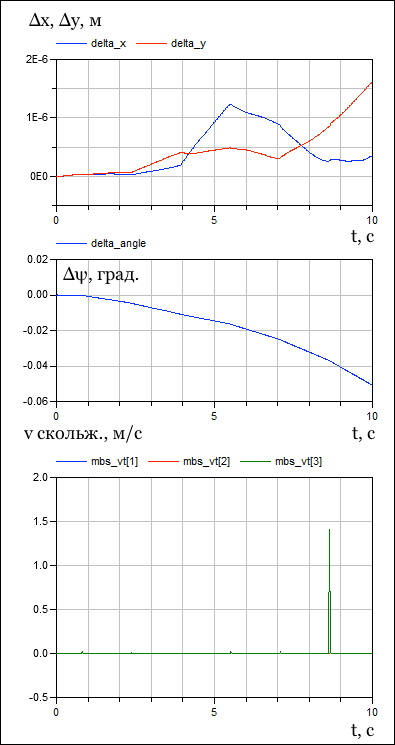
\includegraphics[width=7cm, viewport=0 0 395 745,clip]{content/parts/3_friction/diploma/img/res/comparison_v_0_0_omega_1_frac_1e-3_n_4_time_10s.png} & 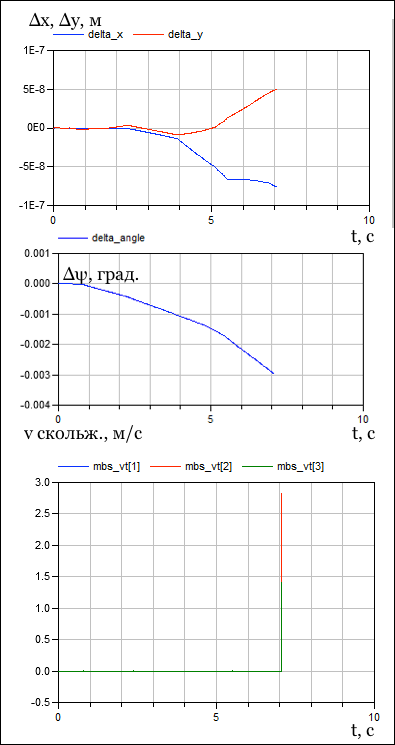
\includegraphics[width=7cm, viewport=0 0 395 745,clip]{content/parts/3_friction/diploma/img/res/comparison_v_0_0_omega_1_frac_1e-4_n_4_time_10s.png}\\
\eta = 0,001, v_0 = 0, \omega_0 = 1 & \eta = 0,0001, v_0 = 0, \omega_0 = 1\\
\end{array}\end{equation*}\end{center}
\end{figure*}

\begin{figure*}[p]
\begin{center}\begin{equation*}\begin{array}{cc}
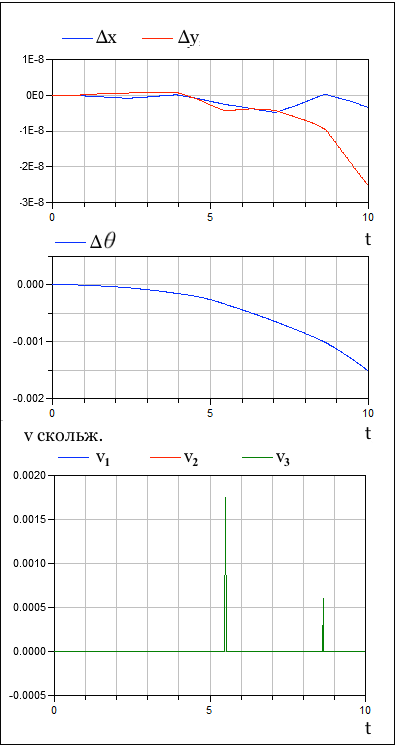
\includegraphics[width=7cm, viewport=0 0 395 745,clip]{content/parts/3_friction/diploma/img/res/comparison_v_0_0_omega_1_frac_1e-5_n_4_time_10s.png} & 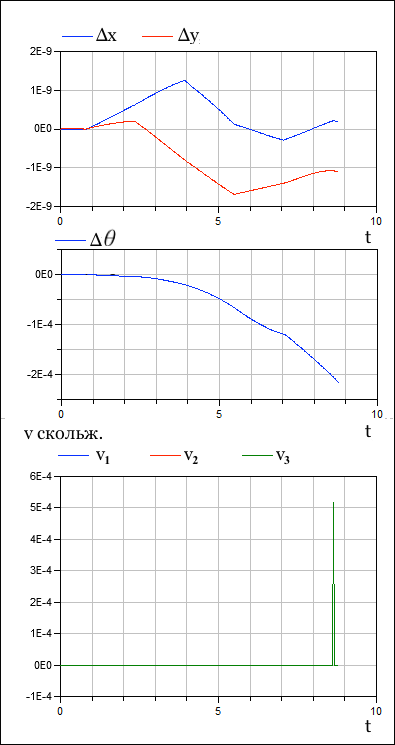
\includegraphics[width=7cm, viewport=0 0 395 745,clip]{content/parts/3_friction/diploma/img/res/comparison_v_0_0_omega_1_frac_1e-6_n_4_time_10s.png}\\
\eta = 10^{-5}, v_0 = 0, \omega_0 = 1 & \eta = 10^{-6}, v_0 = 0, \omega_0 = 1\\
\end{array}\end{equation*}\end{center}
\end{figure*}

\begin{figure*}[p]
\begin{center}\begin{equation*}\begin{array}{cc}
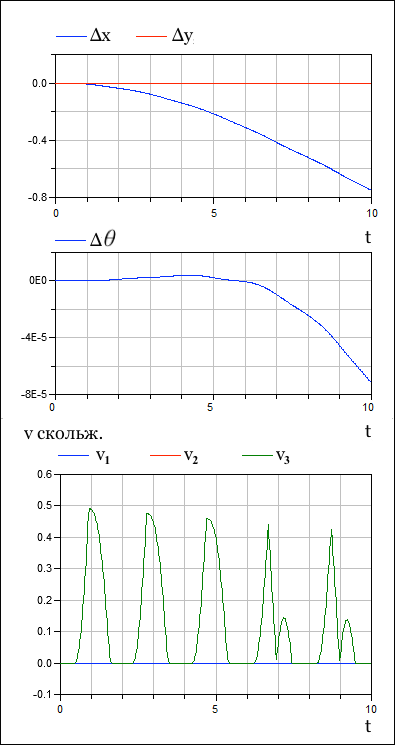
\includegraphics[width=7cm, viewport=0 0 395 745,clip]{content/parts/3_friction/diploma/img/res/comparison_v_1_0_omega_0_frac_1e-1_n_4_time_10s.png} & 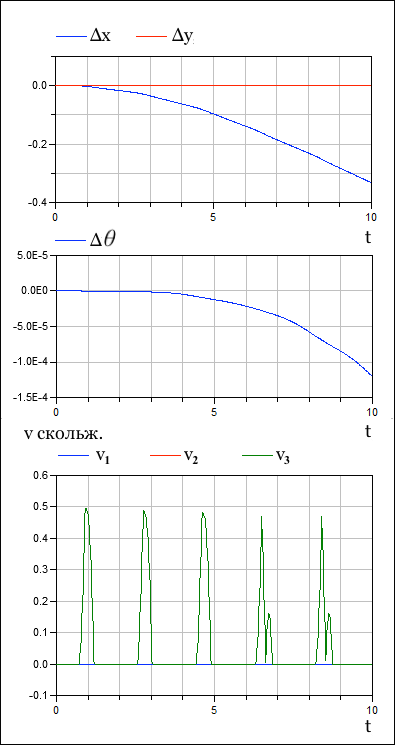
\includegraphics[width=7cm, viewport=0 0 395 745,clip]{content/parts/3_friction/diploma/img/res/comparison_v_1_0_omega_0_frac_1e-2_n_4_time_10s.png}\\
\eta = 0,1, v_0 = 1, \omega_0 = 0 & \eta = 0,01, v_0 = 1, \omega_0 = 0\\
\end{array}\end{equation*}\end{center}
\end{figure*}

\begin{figure*}[p]
\begin{center}\begin{equation*}\begin{array}{cc}
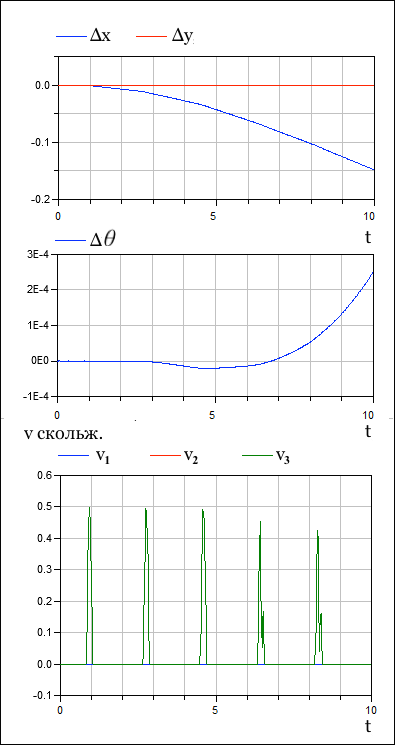
\includegraphics[width=7cm, viewport=0 0 395 745,clip]{content/parts/3_friction/diploma/img/res/comparison_v_1_0_omega_0_frac_1e-3_n_4_time_10s.png} & 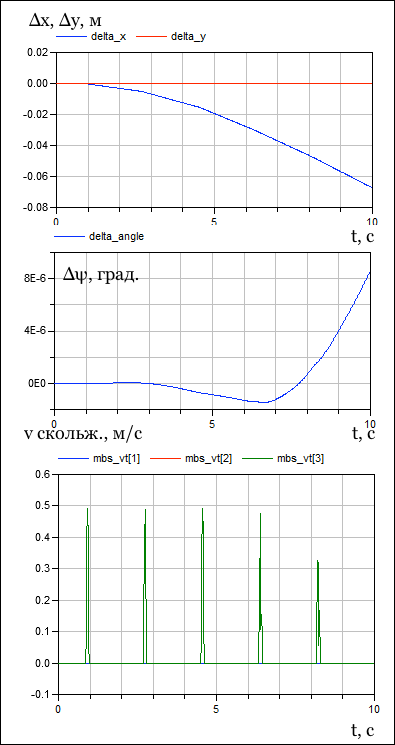
\includegraphics[width=7cm, viewport=0 0 395 745,clip]{content/parts/3_friction/diploma/img/res/comparison_v_1_0_omega_0_frac_1e-4_n_4_time_10s.png}\\
\eta = 0,001, v_0 = 1, \omega_0 = 0 & \eta = 0,0001, v_0 = 1, \omega_0 = 0\\
\end{array}\end{equation*}\end{center}
\end{figure*}


\end{document}


